\documentclass[conference]{IEEEtran}
\IEEEoverridecommandlockouts
% The preceding line is only needed to identify funding in the first footnote. If that is unneeded, please comment it out.
\usepackage{cite}
\usepackage{amsmath,amssymb,amsfonts}
\usepackage{algorithmic}
\usepackage{graphicx}
\usepackage{textcomp}
\usepackage{xcolor}
\usepackage{footnote}
\usepackage{multicol}
\usepackage{float}
\usepackage{url}[hyphens]
\usepackage[acronym, nonumberlist]{glossaries}

\def\BibTeX{{\rm B\kern-.05em{\sc i\kern-.025em b}\kern-.08em
    T\kern-.1667em\lower.7ex\hbox{E}\kern-.125emX}}
\begin{document}

\title{A virtual NDN environment for sharing objects across data infrastructures
}

\author{\IEEEauthorblockN{1\textsuperscript{st} Given Name Surname}
\IEEEauthorblockA{\textit{dept. name of organization (of Aff.)} \\
\textit{name of organization (of Aff.)}\\
City, Country \\
email address}
\and
\IEEEauthorblockN{2\textsuperscript{nd} Given Name Surname}
\IEEEauthorblockA{\textit{dept. name of organization (of Aff.)} \\
\textit{name of organization (of Aff.)}\\
City, Country \\
email address}
\and
\IEEEauthorblockN{3\textsuperscript{rd} Given Name Surname}
\IEEEauthorblockA{\textit{dept. name of organization (of Aff.)} \\
\textit{name of organization (of Aff.)}\\
City, Country \\
email address}
\and
\IEEEauthorblockN{4\textsuperscript{th} Given Name Surname}
\IEEEauthorblockA{\textit{dept. name of organization (of Aff.)} \\
\textit{name of organization (of Aff.)}\\
City, Country \\
email address}
\and
\IEEEauthorblockN{5\textsuperscript{th} Given Name Surname}
\IEEEauthorblockA{\textit{dept. name of organization (of Aff.)} \\
\textit{name of organization (of Aff.)}\\
City, Country \\
email address}
\and
\IEEEauthorblockN{6\textsuperscript{th} Given Name Surname}
\IEEEauthorblockA{\textit{dept. name of organization (of Aff.)} \\
\textit{name of organization (of Aff.)}\\
City, Country \\
email address}
}

\maketitle

% ---------- OVERALL TODO LIST ------------
% minimize references list (can be done after draft is done - not a prio now)
% keep all sections to their essentials (leave out explaining things ieee people already know about)
% minimize sections (compared to our thesis); best to have only e.g.: intro, related work, architecture and design, conclusions
% incorporate cas his work - can be done in architecture - where current pid work in our thesis is just a simple poc, cas his work is more a workable implementation (probably skip our poc for most parts)
% since 2 columns are used, more paragraphs could be added for readability


\begin{abstract}
% can be shortened too, perhaps just one paragraph
Research clouds contain diverse and large datasets, this data is published by the use of \glspl{pid}. The traditional network approach for data transmissions are done with host-to-host connections (IP), where every data request from the consumer is answered with a data transfer from the source (the producer). This approach can potentially cause congestion and delays with many data consumers. \gls{ndn} is a data centric approach where unique data, once requested, may be stored on intermediate hops in the network. Consecutive requests for that unique data object are then made available by these intermediate hops (caching). This approach distributes traffic load more efficient and reliable compared to host-to-host connection oriented techniques.

The \glspl{pid} are used by data providers within these data infrastructures for sharing and identifying digital objects. In order to create \gls{pid} and \gls{ndn} integration, a translation between the different naming schemas is needed. This paper proposes a solution for accessing and sharing digital objects with different \gls{pid} schemas over a networked environment using \gls{doip} and \gls{ndn}. Furthermore, a solution is proposed to plan and deploy an \gls{ndn} with a scalable method for cloud environments.
\end{abstract}

\begin{IEEEkeywords}
Named Data Networking, Persistent Identifier, Digital Object Interface Protocol, FAIRness, Network Functions Virtualization
\end{IEEEkeywords}

\section{Introduction}
% what is the problem
% where does this problem stem from?
% TODO: add figures

Research clouds such as proposed in the \gls{eosc} will offer Europe's 1.7 million researchers and 70 million science and technology professionals the means to store, share and re-use large volumes of information generated by the big data revolution. Research clouds publish datasets from distributed sources, identified by a \gls{pid}. These datasets are not accessed via e.g. a simple web portal like traditional internet objects on the web. Instead these requests are processed by e.g. a data catalog of the federated research cloud. Therefore, research clouds face the challenge of identifying distributed data in a federated cloud, provide data provenance and provide a scalable service to serve many users that request large datasets.

Furthermore, research clouds face a trend of increased data production and consumption, which is expected to grow. This general trend in research clouds calls for a data distribution solution that better supports the scale and complexity. An example of such a research cloud is SeaDataNet, which is a distributed marine data infrastructure network for managing the large and diverse data sets collected by the oceanographic fleets and the automatic observation systems. Their aim is to advance and increase the usage of SeaDataNet's services by adopting cloud and high performance computing technology for better performance.

\begin{figure}[H]
\centering
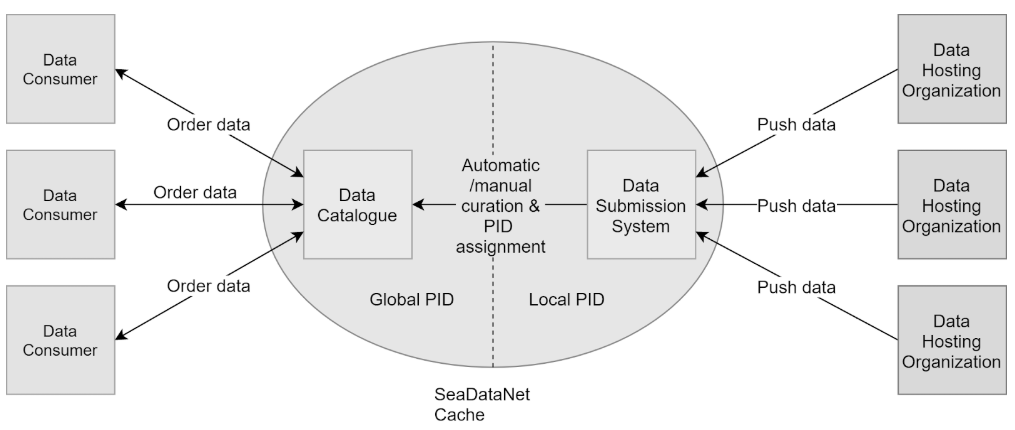
\includegraphics[width=\columnwidth]{images/SDC_current.png}
\caption{SeaDataNet's current infrastructure.}
\label{fig:sdc_cur}
\end{figure}

% add the figures here as well as reference point

Introducing the architecture in figure \ref{fig:sdc_cur} into an NDN is not solved yet. Multiple data providers need to be hosted, which potentially use different PID schemes. \gls{naas4pid} is an extension of \gls{ndn} which allows it to interoperate with \glspl{pid} and is used by SeaDataNet. \gls{naas4pid} adds an additional system layer which translates PIDs to NDN names and optimizes and manages the virtual NDN overlay in cloud or other e-infrastructures. However, \gls{naas4pid} currently only supports a single \gls{pid} provider.


% Add some connection to interoperability needs

\section{Challenges and related work}
% which challenges does this problem bring?
% what has already been done?
% deploying an ndn is a challenge, why? what could help to guide such a deployment? briefly mention tosca and mccabe. also highlight that this paper is devided into 2 parts.


\subsection{PID interoperability}
\label{introduction-pid}
% needs to be trimmed, only the essentials needed
In 2014, Karakannas researched the efficiency of \gls{icn} for delivering big data with \glspl{pid} \cite{icn-bd}. The research proposed a mapping architecture for resolving \glspl{pid} to \gls{icn} names. Karakannas proposed to use a \gls{pid} to \gls{ndn} mapping server for every \gls{pid} type instead of implementing the translation on the clients browser.

In 2017, Mousa researched the fetching and sharing of \gls{doi} objects with \gls{icn} such as \gls{ndn}. The researcher's approach focused only on \gls{doi} identified objects within \gls{ndn}'s. The researcher explained that the difference in \gls{ndn} naming of different \gls{pid} providers must be taken into account, such that the correct prefix is used within \gls{ndn} to identify specific \gls{pid} types. For example, using the prefix \texttt{/doi} within \gls{ndn} for \gls{doi} identified objects. In the researcher's design, the translation happens in the consumers browsers. The consumer has the choice to either request the digital object by its \gls{ndn} name or \gls{pid} \cite{ndn-app-aware}.

Zhao et al. continued the research done by Karakannas \cite{icn-bd} and Mousa \cite{ndn-app-aware} and proposed an architecture to map \glspl{pid} into the naming schema of \gls{ndn}. Their proposed solution is named \gls{naas4pid} and supports one \gls{pid} type. This solution is composed out of three key components \cite{koulouzis2018information}:
\begin{itemize}
  \item \gls{pid}2\gls{ndn} gateway.
  \begin{itemize}
        \item Primarily responsible for resolving \glspl{pid} to \gls{ndn} names.
  \end{itemize}
  \item \gls{ndn}4\gls{pid} router image.
    \begin{itemize}
        \item An \gls{ndn} node that implements a virtualized \gls{ndn} router.
    \end{itemize}
  \item \gls{ndn}4\gls{pid} manager.
    \begin{itemize}
        \item Automates the management of the \gls{ndn} overlay in\newline cloud or e-infrastructure.
    \end{itemize}
\end{itemize}


\subsection{Named Data Networking}
% needs to be trimmed a bit as well
NDN is not yet implemented on a large scale, with the exception of several large testbeds. In order to plan an \gls{ndn}, it would be necessary to know what works and does not work. However, there is sufficient research available that focused on particular design choices of \gls{ndn}. Research done by Lim et al. at a large existing testbed located in the USA highlighted a few lessons learned \cite{lim2018ndn, ndn-testbed-status}. Lim et al. setup the first intercontinental \gls{ndn} testbed with the intent to see the benefits for big science. They concluded that \gls{ndn} provided performance improvements compared to classical climate data delivery techniques based on TCP/IP. \gls{ndn} over TCP demonstrated a more reliable and faster performance compared to UDP. This was due to the allowance of larger dynamic window sizes and congestion control in TCP. Native \gls{ndn} congestion control is still an open research area \cite{ren2016congestion}, as of writing this paper, no proposal has been implemented.

The performance benefits of \gls{ndn} concluded by Lim et al. correlates with research done by Shannigrahi et al. at the USA-based large hadron collider network \cite{shannigrahi2015named}. The researchers achieved a 71\% reduction in the average delay per data chunk compared to a no-caching case. They conducted \gls{ndn} caching simulations \cite{shannigrahi2017request}, where they concluded that a small cache of several gigabytes reduces the network load. However, as expected, increasing the cache towards 1TB reduced the network load even further. However, this reduction of load was not proportional to the cache size. They concluded in their research that a 1GB \gls{ndn} cache at the edge of the \gls{ndn} can already significantly improve data distribution and reduce the network load. The average file size in use was 1.3GB.

Furthermore, in \gls{ndn} several caching, cache replacement and forwarding strategies can be used to fine-tune performance. Koulouzis et al. researched these strategies and concluded that the `leave copy everywhere' caching strategy provided the best performance ratio between cache size to data object size for generic data usage \cite{koulouzis2018information}. However, `leave copy down' and `leaving copies with probability' performed best for delivering big data objects. Koulouzis et al. also concluded that the ascending ordering of data objects enhances network performance when combined with the `least recently used' caching strategy. This was concluded based on observations that if large objects were requested first, the cache replacement algorithm would make room by overwriting files already in the cache, resulting in cache misses. When small files were requested first, more cache hits were measured. As for cache size, the researchers recommended a cache size at least twice the size of the biggest data object in the network \cite{koulouzis2018information}.

Yuan et al. \cite{yuan2012scalable} researched the performance of \gls{ndn} forwarding. They used the \gls{ccnx} application\footnote{\url{https://wiki.fd.io/view/Cicn}} to perform experiments. Their research concluded that packets with long names degraded performance. After profiling the software they measured that the \gls{ndn} name decode operation took 35.46\% of the entire program running time. So et al. \cite{so2013named} developed a method to achieve fixed lookup times with variable length names. In order to achieve this goal they explored the application of hash tables to do name lookup. Furthermore, they explored the possibility to do this in hardware by using a Cisco ASR9000 router with the integrated service module running 64-bit Linux. With their experiments they managed to forward 20Gbps of real \gls{ndn} traffic. Tortelli et al. \cite{tortelli2013performance} researched the effectiveness of two opposite forward strategies; flooding and best-route (with and without caching). Several experiments lead them to the conclusion that there are pros and cons in each forwarding strategy. But that it is difficult to determine the best performing forward strategy.

% \section{Architecture and technical considerations}
% brief intro acting as a glue between the 2 subsections

\section{PID interoperability}
% Discuss briefly the proof of concept architecture of our thesis: simple regex matching to translation function in code
% highlight cas his design and how it extents the work done in our thesis




\section{Planning and deploying an NDN}
% focus on research clouds
% discuss the ndn planning and deployment (nfv, tosca, kubernetes, cloud infra)
% TODO: add figures

% flow of section
% discuss overall objective to solve the problem
% glue mccabe and tosca together
% go through the train of thought of planning and deployment

\subsection{Planning}

\subsubsection{McCabe}
Scalability is defined as capacity to be changed in size or scale. In order to plan an \gls{ndn} with this goal in mind we used McCabe's method. McCabe's book `Network Analysis, Architecture, and Design' \cite{mccabe2010network} is about applying a systems methodology approach towards network design. McCabe's approach consists out of three core phases; analysis, architecture and design. These simple, yet important planning phases in McCabe describe how to make technology and topology decisions in a network, especially for large deployments. These decisions are guided based on inputs for these three core phases, the initial input may be from users and/or from network metrics. Consecutive processes use the output of previous processes as input, thus these processes are interconnected.

\begin{figure}[H]
\centering
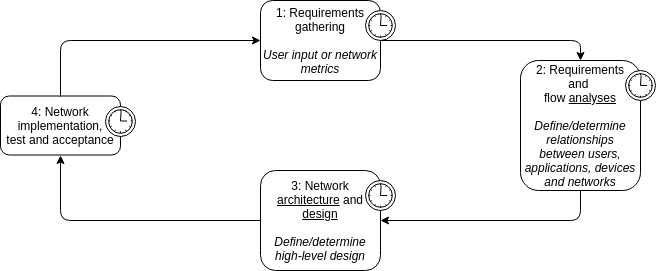
\includegraphics[width=\columnwidth]{images/mccabe-process.png}
\caption{Cyclic and iterative nature of McCabe's processes and phases.}
\label{fig:mccabe-process}
\end{figure}

In figure \ref{fig:mccabe-process} the three core phases are illustrated in \textit{italic} while the processes are in normal text. In order to highlight the core phases by name they are \underline{underlined} in the figure. The first phase (analysis) has as goal to understand the network and potential problems in terms of performance and efficiency in order to determine network requirements. This is done by developing sets of problem statements and objectives that describe what the target network should address. Therefore, historical data from network management (monitoring), requirements gathered from the network users, staff and management are included in the analysis phase. Furthermore, these metrics are then compared to the relationships between users, applications, devices and other networks in order to determine if requirements match with the user and network expectations. The second and third phase (architecture and design) uses the output of the first phase to establish a high-level design of the network. This network design determines which technology and topology choices are justified to improve the network requirements established in the first phase. The fourth process is implementing the design, test if requirements are met and finally accept the implementation. These phases are intended to be iterative and by no means define a final architecture design. This is due to the fact that requirements, technology and user behavior can change and with that the network design.

The following analysis provides a starting baseline for the high-level network design. As discussed in the related work section, several key scalability and performance metrics were addressed. It was concluded that TCP provided the most satisfying performance when compared to UDP. Furthermore, there are several \gls{ndn} strategies to choose from. The `leave copy everywhere' cache decision strategy and the `least recently used' cache replacement strategy were considered to be the overall best performing choices. However, for the forward strategies there was no decisive conclusion on which a selection could be based on. Therefore, we will use the default forwarding strategy; best-route. In terms of cache size, Koulouzis et al. recommends a cache size twice the size of the largest data object residing in the used repositories \cite{koulouzis2018information}. The data catalogue or registry system provides metadata of digital objects, where the size and \gls{pid} type is available. This information may be used to sort the files in the (research cloud) catalogue by maximum size. The performance configurations mentioned can be configured in the \texttt{nfd.conf} file of the \gls{cxx} application. \gls{cxx} is one of the most mature software implementations of \gls{ndn} and therefore used in our design. Other performance optimization solutions which were mentioned in the related work section require changes in the source-code. These source-code optimizations were not made public or are not yet integrated in existing software and therefore were not used.

% This perhaps could be left out
% The following hardware requirements were determined based on the Kubernetes and NDN\footnote{\url{https://github.com/named-data/ndn-cxx}} software documentation, the problem statement described in the introduction and related work. For VM memory requirements, 8-12GB and 2 CPUs or more are recommended. This was determined based on the recommended system requirements for Kubernetes and the fact that the use case may be I/O intensive. Therefore, I/O caching in memory benefits performance. In order to have sufficient disk space to cache \gls{ndn} data objects, install software, store logs and containers, a minimum of 100GB of storage is recommended.

\subsubsection{NFV}
A requirement is flexible scalability, this will be addressed by deploying and managing \gls{ndn} in an \gls{nfv}-style. Therefore, \gls{ndn} will be deployed as virtual functions and managed centrally via Kubernetes. \gls{nfv} is a network architecture concept which uses virtualization to create and manage higher level network functions, as software, on commodity hardware. These functions may be interconnected to create a network service such as load-balancers, firewalls or intrusion detection. This architecture differs from traditional network architectures, where network functions are provided by hardware devices. \gls{nfv} provides the ability to easily duplicate network functionality and expand the network locally or into other data centers. \gls{nfv} is usually managed by an orchestrator to automate deployment, thus providing less overhead than traditional network management with hardware devices.

% missing gap; how does kubernetes fit in here - can be a short paragraph
% describe why and how it's useful to have ndn in containers and thus nfv - also highlight the usefulness of kubernets in this

\begin{figure}[H]
\centering
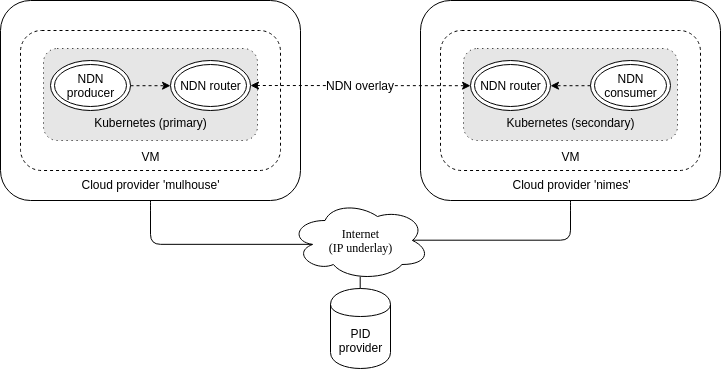
\includegraphics[width=\columnwidth]{images/high-level-network-design.png}
\caption{High-level network design.}
\label{fig:high-level-network-design}
\end{figure}

\begin{figure*}[ht]
\centering
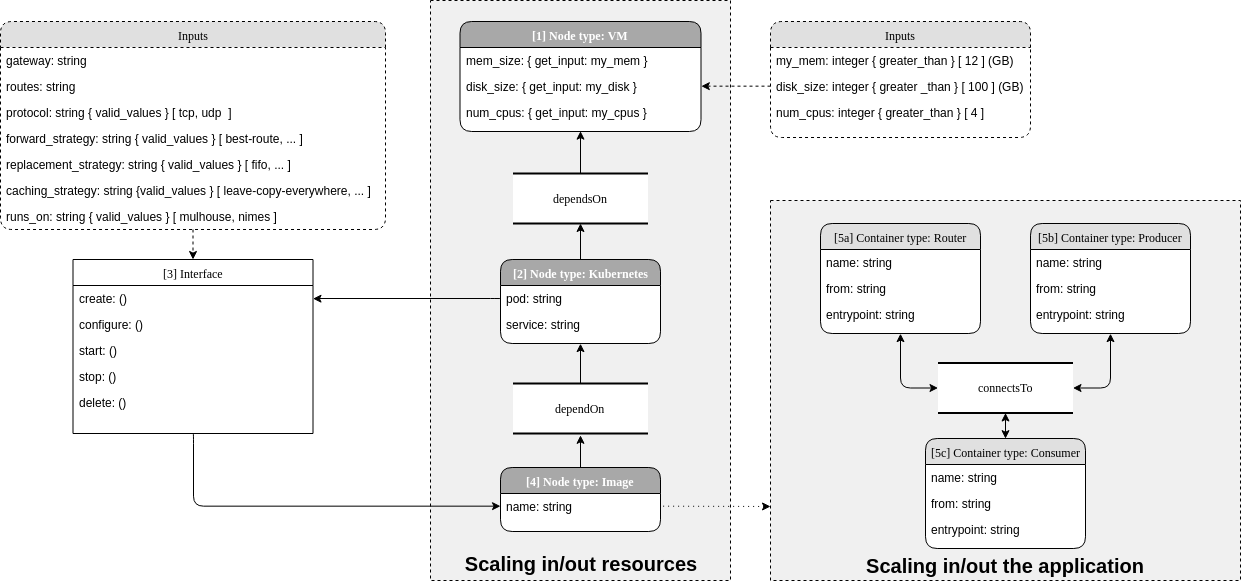
\includegraphics[width=\textwidth]{images/tosca-diagram.png}
\caption{TOSCA diagram.}
\label{fig:tosca-diagram}
\end{figure*}

Virtualization allows for flexible allocation of cloud resources via VMs while scalability of software applications can be realized by the use of containers in a \gls{nfv}-style. If more cloud resources are required, then this can be done by deploying more VMs. Furthermore, if needed, VMs can be deployed in specific geographically located cloud providers, expanding the data distribution availability. The virtual \gls{ndn} functions running inside these cloud providers, can then provide locally cached copies of data objects. And thus providing data distribution which lowers the chance of network congestion. In figure \ref{fig:high-level-network-design} we illustrate our high-level network design. In this illustration there are two conceptual cloud providers; 'mulhouse' and 'nimes'. These two nodes each are equipped with 12GB RAM and an Intel Xeon CPU E3-1240L v5 @ 2.10GHz with 1TB disks. In both of these conceptual cloud providers a VM will be deployed in order to allocate the resources needed.


% tosca part might be slimmed down
\subsubsection{TOSCA}
The heterogeneous nature in cloud environments can make deployment automation and management complicated. \gls{tosca} \cite{tosca-standard} is a method to describe the deployment and management of a cloud infrastructure based on reusable templates. These descriptions are then used by orchestrators to facilitate the deployment. SeaClouds \cite{seaclouds-website} (\gls{fp7} funded project), not to be confused with SeaDataNet, is a research cloud that already manages infrastructures based on \gls{tosca}. Brogi et al. \cite{brogi2015adaptive} concluded that SeaClouds can now realize their multiple cloud infrastructures in an automated arrangement with central coordination, deployment and management without the need to make custom deployment strategies for each cloud environment. Furthermore, several large companies such as Google, Red Hat, Canonical and IBM are also involved with the development of TOSCA, signifying that broader adoption may follow in the future.

\gls{drip} is currently a TOSCA-compatible prototype which uses the open cloud computing interface and currently supports EC2 \cite{amazon-website}, \gls{egi} FedCloud \cite{egi-website} and \gls{exogeni} \cite{exogeni-website} clouds. Furthermore, \gls{drip} also supports Ansible playbooks \cite{ansible-website} for configuration management and contains a deployment agent for e.g. Kubernetes. This results into a portable (can be run by any orchestrator that understands TOSCA) and automated method (implementation carried out by an orchestrator) of infrastructure management. This allows interoperability and reusability of \gls{tosca} template descriptions on different cloud providers. Reusability of templates is made possible by using variables to substitute e.g. IPs or hostnames. These variables can be retrieved with the `get\_attribute' function and can be declared by a reference node or relationship template \cite{tosca-attributes}.

TOSCA template descriptions consist out of the following core components; nodes, relationships and interfaces. Nodes can be a host, container or VM and are connected to each other through relationships such as `dependsOn', `hostedOn' and `connectsTo'. These relationships can be used to describe that a VM is `hosted on' a host (e.g. a bare metal machine). Or that a set of containers 'depend on' each other for functionality and 'connect to' e.g. a database. Such as a containerized web application that requires a database, facilitated by another container. Interfaces are used to control the life cycle of a component and consist as a set of hooks to trigger actions, these actions are create, configure, start, stop or delete. These hooks can be triggered to e.g. configure and create containers, stop or start a service or do system maintenance such as delete artifacts after a service is stopped. Furthermore, constraints can be set for the input values in these template descriptions. These can be e.g. that the amount of CPU's should be defined with integers and should contain a value more than one. However, the orchestrator is responsible for verifying these constraints, \gls{tosca} is merely a means to describe components in an infrastructure.

In figure \ref{fig:tosca-diagram}, a \gls{tosca} diagram is illustrated. This diagram represents an abstract template description of the \gls{tosca} relationships, in which the grey rectangular boxes are the core scalability factors. \gls{tosca} consists out of several types; nodes, relationships and interfaces. The scaling properties are highlighted in the rectangular areas. The left area, highlighted as `scaling in/out resources' contains a dependency chain of several virtual \gls{ndn} functions. This dependency chain is also depicted numerically.

Before a pod (container) can be deployed on Kubernetes (step 2 to 5), a VM needs to exist (step 1). This is described by the `dependsOn' relationship. Furthermore, with the requirements defined, input constraints are described. These constraints are used by the orchestrator to make sure that the \gls{ndn} infrastructure has sufficient resources available to operate. Once a VM is deployed, the dependency for Kubernetes is satisfied, thus Kubernetes can then be setup (step 2). Kubernetes can then deploy pods by the use of interfaces (step 3). These interfaces feed the containers with environment variables such as the gateway, a list of routes, the transport protocol for \gls{ndn}, the \gls{ndn} strategies and on which Kubernetes node this pod should run. The environment variables are given to the interface via the \gls{tosca} inputs. These environment variables are then used by scripts that run inside the pods to setup \gls{ndn}. Several constraints are set for these environment variables such as which valid transport protocols can be used for \gls{ndn}, which \gls{ndn} strategies are valid and which nodes are available. These constraints are defined with e.g. `valid\_values' or `greater\_than' definitions. These constraints help to guide the orchestrator to verify the inputs that are given for the template description. As illustrated in the second gray area `scaling in/out the application', several pods can be instantiated (step 5a, 5b and 5c) from the image (step 4). These pods enable the virtual \gls{ndn} functions. These pods establish the \gls{ndn} and therefore are connected via the `connectsTo' relationship. This network expands over to other Kubernetes nodes in the cluster by the use of the Kubernetes built-in overlay network.

\subsection{NDN deployment as NFV}
% trim - most can be merged with discussion
% add sed command to substitute config lines in nfd.conf
The orchestrators mentioned when combined with a \gls{tosca} parser are still in a prototype phase. Therefore, in our proof of concept we deployed the VMs and Kubernetes nodes manually. In practice the life cycle of also the Kubernetes pods are managed by a \gls{tosca} orchestrator. Without having a \gls{tosca}-ready orchestrator available, steps 2 through 5 in figure \ref{fig:tosca-diagram} were be carried out by Kubernetes exclusively. This was done by defining the configuration properties\footnote{\url{https://github.com/AquaL1te/rp2/blob/master/Kubernetes/expanded-cluster.yml}} of the pods manually. These properties include the \gls{ndn} function name, e.g. router, producer or consumer. And also includes the routes (NDN prefixes) and the associated \gls{ndn} face with the transport protocol to use (TCP or UDP). These parameters were then inserted into the \gls{ndn} \gls{fib} by the scripts that were executed inside the pod\footnote{\url{https://github.com/AquaL1te/rp2/blob/master/Docker/producer/docker-entrypoint.sh}}. The \gls{ndn} strategies were also configured by these scripts. Furthermore, if it is not defined where a pod should be running, Kubernetes will make this decision itself, based on the known resources in the Kubernetes cluster. If for example a Kubernetes node has more memory to spare than other nodes, then Kubernetes will likely decide to spawn the pod there. This Kubernetes node could potentially run in a cloud provider, located in another geographical area. Since the purpose is to provide data distribution through the use of \gls{ndn}, locality becomes a key factor. Therefore, a pod is specifically assigned to a Kubernetes node in order to provide in-network caching in a specific geographical area.

The methods discussed offer a combined way to plan and deploy a data distribution network. McCabe can be used to methodologically adjust the environment to match performance requirements. For the size of this proof of concept the McCabe method is extra overhead. However, the proof of concept is only used to demonstrate the train of thought. The methods discussed can be applied to larger deployments where the McCabe method will be more valuable.

\section{Discussion}
% discuss novelty (can be taken from conclusion, discussion and parts of future work from our thesis)
Furthermore, the \gls{ndn} infrastructure life cycle can be managed from Kubernetes. Our proof of concept lacks a \gls{tosca}-ready orchestrator. Therefore, scaling in or out resources to other cloud providers is not demonstrated. However, scaling in or out the \gls{ndn} application is demonstrated. This method allows to reconfigure an \gls{ndn} infrastructure in \gls{nfv}-style by interacting with Kubernetes as the orchestrator. Therefore, the YAML configuration of Kubernetes acts as the \gls{tosca} template description and Kubernetes, which executes this configuration, acts as the orchestrator. In practice the Kubernetes configuration would be generated based on the \gls{tosca} template descriptions and e.g. \gls{drip} would act as the orchestrator. In effect, the \gls{ndn} containers are spawned as \glspl{nfv} which provides scalable management of the \gls{ndn}. These \gls{ndn} \glspl{nfv} may be deployed on a continental or global scale, facilitating a managed distribution network.

In contrast, if \gls{ndn} was deployed without the discussed methods, an alternative would be to have a custom deployments for each cloud environment. Which does not scale in terms of manageability and may create inconsistent deployments and errors. Therefore, that approach also realizes a data distribution network by the use of \gls{ndn}, but does not scale in terms of management and deployment.



\section*{Acknowledgment}
% our thesis + zhiming + cas

% \section*{References}
% max 8, probably naas4pid, our thesis, and others
\newacronym{pid}{PID}{Persistent Identifier}
\newacronym{eosc}{EOSC}{European Open Science Cloud}
\newacronym{ndn}{NDN}{Named Data Networking}
\newacronym{icn}{ICN}{Information Centric Networking}
\newacronym{cmmap}{CMMAP}{Center for Multiscale Modeling of Atmospheric Processes}
\newacronym{cmip}{CMIP5}{Coupled Model Intercomparison Project}
\newacronym{uri}{URI}{Uniform Resource Identifier}
\newacronym{url}{URL}{Uniform Resource Locator}
\newacronym{urn}{URN}{Uniform Resource Name}
\newacronym{doi}{DOI}{Digital Object Identifier}
\newacronym{purl}{PURL}{Persistent Uniform Resource Locator}
\newacronym{ark}{ARK}{Archival Resource Key}
\newacronym{tosca}{TOSCA}{Topology and Orchestration Specification for Cloud Applications}
\newacronym{drip}{DRIP}{Dynamic Real-time Infrastructure Planner}
\newacronym{cnri}{CNRI}{Corporation for National Research Initiatives}
\newacronym{fib}{FIB}{Forwarding Information Base}
\newacronym{pit}{PIT}{Pending Interest Table}
\newacronym{cs}{CS}{Content Store}
\newacronym{n2t}{N2T}{Names to Things}
\newacronym{ospfn}{OSPFN}{Open Shortest Path First for NDN}
\newacronym{ghr}{GHR}{Global Handle Registry}
\newacronym{ghs}{GHS}{Global Handle System}
\newacronym{dtr}{DTR}{Data Type Registry}
\newacronym{ra}{RA}{Registration Authority}
\newacronym{idf}{IDF}{International DOI Foundation}
\newacronym{nlsr}{NLSR}{Named-data Link State Routing}
\newacronym{cs3}{CS3}{Cloud Storage Synchronization and Sharing Services}
\newacronym{cdn}{CDN}{Content Delivery Network}
\newacronym{nfv}{NFV}{Network Functions Virtualization}
\newacronym{isbn}{ISBN}{International Standard Book Number}
\newacronym{gpl}{GPLv3}{General Public License}
\newacronym{ddos}{DDoS}{Distributed Denial of Service}
\newacronym{naas4pid}{NaaS4PID}{NDN-as-a-service for PID data objects}
\newacronym{cxx}{NDN-CXX}{NDN C++ library with eXperimental eXtensions}
\newacronym{ccnx}{CCNx}{Content-Centric Networking}
\newacronym{rfc}{RFC}{Request for Comments}
\newacronym{dona}{DONA}{Digital Object Numbering Authority}
\newacronym{ucs}{UCS}{Universal Coded Character Set}
\newacronym{rdf}{RDF}{Resource Description Framework}
\newacronym{oasis}{OASIS}{Organization for the Advancement of Structured Information Standards}
\newacronym{egi}{EGI}{European Grid Infrastructure}
\newacronym{exogeni}{ExoGENI}{Exo Global Environment for Network Innovation}
\newacronym{fp7}{EU FP7}{European Seventh Framework Programme}
\newacronym{do}{DO}{Digital Object}
\newacronym{dcx}{DCX}{Dublin Core}
\newacronym{anp}{ANP}{Algemeen Nederlands Persbureau}
\newacronym{nr}{NR}{National Resolver}
\newacronym{ir}{IR}{Institutional Repository}
\newacronym{doip}{DOIP}{Digital Object Interface Protocol}
\newacronym{fairness}{FAIRness}{Findability, Accessibility, Interoperability and Re-usability}

\bibliographystyle{./bibliography/IEEEtran}
\bibliography{./bibliography/IEEEabrv,./bibliography/IEEEexample}

\end{document}